% $Id: template.tex 11 2007-04-03 22:25:53Z jpeltier $

\documentclass{vgtc}                          % final (conference style)

%% These few lines make a distinction between latex and pdflatex calls and they
%% bring in essential packages for graphics and font handling.
%% Note that due to the \DeclareGraphicsExtensions{} call it is no longer necessary
%% to provide the the path and extension of a graphics file:
%% \includegraphics{diamondrule} is completely sufficient.
%%
\ifpdf%                                % if we use pdflatex
  \pdfoutput=1\relax                   % create PDFs from pdfLaTeX
  \pdfcompresslevel=9                  % PDF Compression
  \pdfoptionpdfminorversion=7          % create PDF 1.7
  \ExecuteOptions{pdftex}
  \usepackage{graphicx}                % allow us to embed graphics files
  \DeclareGraphicsExtensions{.pdf,.png,.jpg,.jpeg} % for pdflatex we expect .pdf, .png, or .jpg files
\else%                                 % else we use pure latex
  \ExecuteOptions{dvips}
  \usepackage{graphicx}                % allow us to embed graphics files
  \DeclareGraphicsExtensions{.eps}     % for pure latex we expect eps files
\fi%

%% it is recomended to use ``\autoref{sec:bla}'' instead of ``Fig.~\ref{sec:bla}''
\graphicspath{{figures/}{pictures/}{images/}{./}} % where to search for the images

\usepackage{microtype}                 % use micro-typography (slightly more compact, better to read)
\PassOptionsToPackage{warn}{textcomp}  % to address font issues with \textrightarrow
\usepackage{textcomp}                  % use better special symbols
\usepackage{mathptmx}                  % use matching math font
\usepackage{times}                     % we use Times as the main font
\renewcommand*\ttdefault{txtt}         % a nicer typewriter font
\usepackage{cite}                      % needed to automatically sort the references
\usepackage{tabu}                      % only used for the table example
\usepackage{booktabs}                  % only used for the table example
\usepackage{amssymb}
\usepackage{amsmath}
%% We encourage the use of mathptmx for consistent usage of times font
%% throughout the proceedings. However, if you encounter conflicts
%% with other math-related packages, you may want to disable it.

%% If you are submitting a paper to a conference for review with a double
%% blind reviewing process, please replace the value ``0'' below with your
%% OnlineID. Otherwise, you may safely leave it at ``0''.
\onlineid{0}

%% declare the category of your paper, only shown in review mode
\vgtccategory{Research}

%% allow for this line if you want the electronic option to work properly
\vgtcinsertpkg

%% In preprint mode you may define your own headline.
%\preprinttext{To appear in an IEEE VGTC sponsored conference.}

%% Paper title.

\title{Visualization of Optimization Algorithms}

%% This is how authors are specified in the conference style

\author{Marco Morais\thanks{e-mail: mmorais2@illinois.edu}}
\affiliation{\scriptsize UIUC}

%% Abstract section.
\abstract{
Optimization algorithms seek to find the best solution $x^{*}$ from a set S such that $f(x^{*}) \leq f(x)$ for all $x$ in S. For this project we describe and implement a handful of optimization algorithms, evaluate their performance on some well known test functions, and create visualizations to build some intuition and verify their function. Finally, we perform a comparative analysis between algorithms using repeated trials on these test functions in order to draw broader conclusions.%
} % end of abstract

\CCScatlist{
  \CCScatTwelve{Human-centered computing}{Visualization}{Visualization application domains}{Scientific visualization};
  \CCScatTwelve{Mathematics of computing}{Mathematical analysis}{Mathematical optimization}{Continuous optimization}
}

%%%%%%%%%%%%%%%%%%%%%%%%%%%%%%%%%%%%%%%%%%%%%%%%%%%%%%%%%%%%%%%%
%%%%%%%%%%%%%%%%%%%%%% START OF THE PAPER %%%%%%%%%%%%%%%%%%%%%%
%%%%%%%%%%%%%%%%%%%%%%%%%%%%%%%%%%%%%%%%%%%%%%%%%%%%%%%%%%%%%%%%%

\begin{document}

%% The ``\maketitle'' command must be the first command after the
%% ``\begin{document}'' command. It prepares and prints the title block.

%% the only exception to this rule is the \firstsection command
\firstsection{Introduction}

\maketitle

Given a fuction $f: \mathbb{R}^n \rightarrow \mathbb{R}$ and the set $S \in \mathbb{R}^n$ the solution to an optimization problem seeks to find $x^{*} \in S$ such that $f(x^{*}) \leq f(x)$ for all $x$ in S.  The function $f$ is referred to as the objective function and the set $S$ is referred to the as the constraints.

In this project we will examine 4 different algorithms for solving optimization problems. Each algorithm represents a more general class of problem-solving approaches to optimzation.

In order to understand how each algorithm functions as well as appreciate the strengths and weakness, we choose a set of test functions of varying difficulty. These functions are described in the next section.

\section{Test Functions}

\autoref{tab:test_function_class} summarizes the test functions used in the project. Each test function is classified according to criteria given for optimization test functions in Jamil and Yang (2013) \cite{Jamil:2013:CoRR}.

\begin{itemize}
\item Continous
	\begin{itemize}
    	\item A continuous function has a value $f(x)$ for every $x$ in the domain $S$.
	\end{itemize}
\item Differentiable
	\begin{itemize}
    	\item Gradient-based optimization methods require the objective function to be differentiable within the search domain.  Differentiability criteria are similarly restricted.
    	\item Examples of functions that are not differentiable are absolute value functions or functions with asymptote(s).
	\end{itemize}
\item Unimodal vs. Multimodal
	\begin{itemize}
    	\item A unimodal function is either monotonically increasing or decreasing.  As a result, the function has no local minima or maxima.
    	\item Some of the optimization algorithms we investigate use only gradient information to decide on a search direction and are thus guaranteed to find the global minimum of a unimodal function.  Although gradient-based methods can be used on multimodal functions, there is no guarantee that they will find the global minimum.
	\end{itemize}
\item Separability
	\begin{itemize}
    	\item Degree of independence of parameters in the search space.
    	\item Certain kinds of optimization algorithms can exploit separability during their search, but this criteria is unimportant for the algorithms used in this project.
	\end{itemize}
\end{itemize}

\begin{table}[tb]
	\caption{Test Function Classification}
    \label{tab:test_function_class}
	\scriptsize
	\centering
	\begin{tabu}{
	  r
	  *{7}{c}
	  *{2}{r}
	}
  	\toprule
        Test Function & Criteria \\
	\midrule
        Rosenbrock & Continuous, Differentiable, Non-Separable, Unimodal \\
        Goldstein-Price & Continuous, Differentiable, Non-Separable, Multimodal \\
        Bartels-Conn & Continuous, Non-Differentiable, Non-Separable, Multimodal \\
        Egg Crate & Continuous, Differentiable, Separable, Multimodal \\
	\bottomrule
 	\end{tabu}
\end{table}

\subsection{Rosenbrock Function}

The Rosenbrock function \cite{Rosenbrock:1960} shown in \autoref{fig:rosenbrock} is characterized by a parabolic shaped flat valley bounded by steep canyon walls.

\begin{equation}
f(x_1, \cdots, x_D) = \sum_{i}^{D-1} [ 100(x_{i+1} - x_i^2)^2 + (1 - x_i)^2]
\end{equation}

The global minimum is located at $x^* = f(1, \cdots, 1)$ and $f(x^*) = 0$ and labeled with a diamond in \autoref{fig:rosenbrock}.  The domain of the Rosenbrock function used in this project is restricted to (-2,2) along both $x_1$ and $x_2$ dimensions.  There are 12 regularly sampled points superimposed on \autoref{fig:rosenbrock} and labeled as $x_0$ that are used to initialize separate trials of each optimization algorithm.

\begin{figure}[tb]
\centering
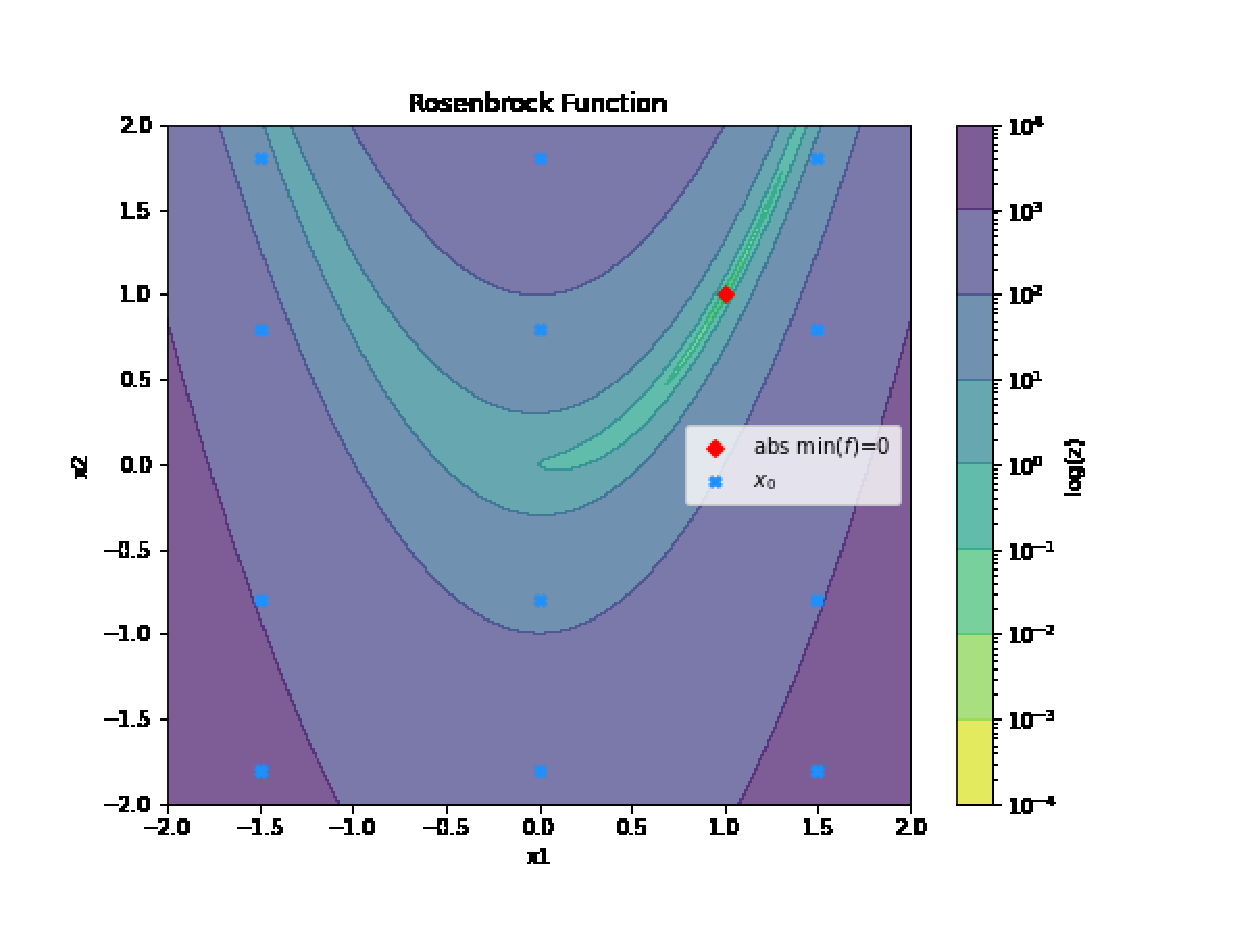
\includegraphics[width=\columnwidth]{figures/pictures/images/rosenbrock-plot2d.eps}
\caption{Rosenbrock Function}
\label{fig:rosenbrock}
\end{figure}

\subsection{Goldstein-Price Function}

The Goldstein-Price function \cite{Goldstein:1971} shown in \autoref{fig:goldstein_price} has a single global minimum, but many local minima and several orders of magnitude difference in range.

\begin{equation}
\begin{split}
f(x_1, x_2) = [1 + (x_1 + x_2 + 1)^2 \\
(19 - 14 x_1 + 3 x_1^2 - 14 x_2 + 6 x_1 x_2 + 3 x_2^2)] \\
\times [30 + (2 x_1 - 3 x_2)^2 \\
(18 - 32 x_1 + 12 x_1^2 + 48 x_2 - 36 x_1 x_2 + 27 x_2^2)]
\end{split}
\end{equation}

\begin{figure}[tb]
\centering
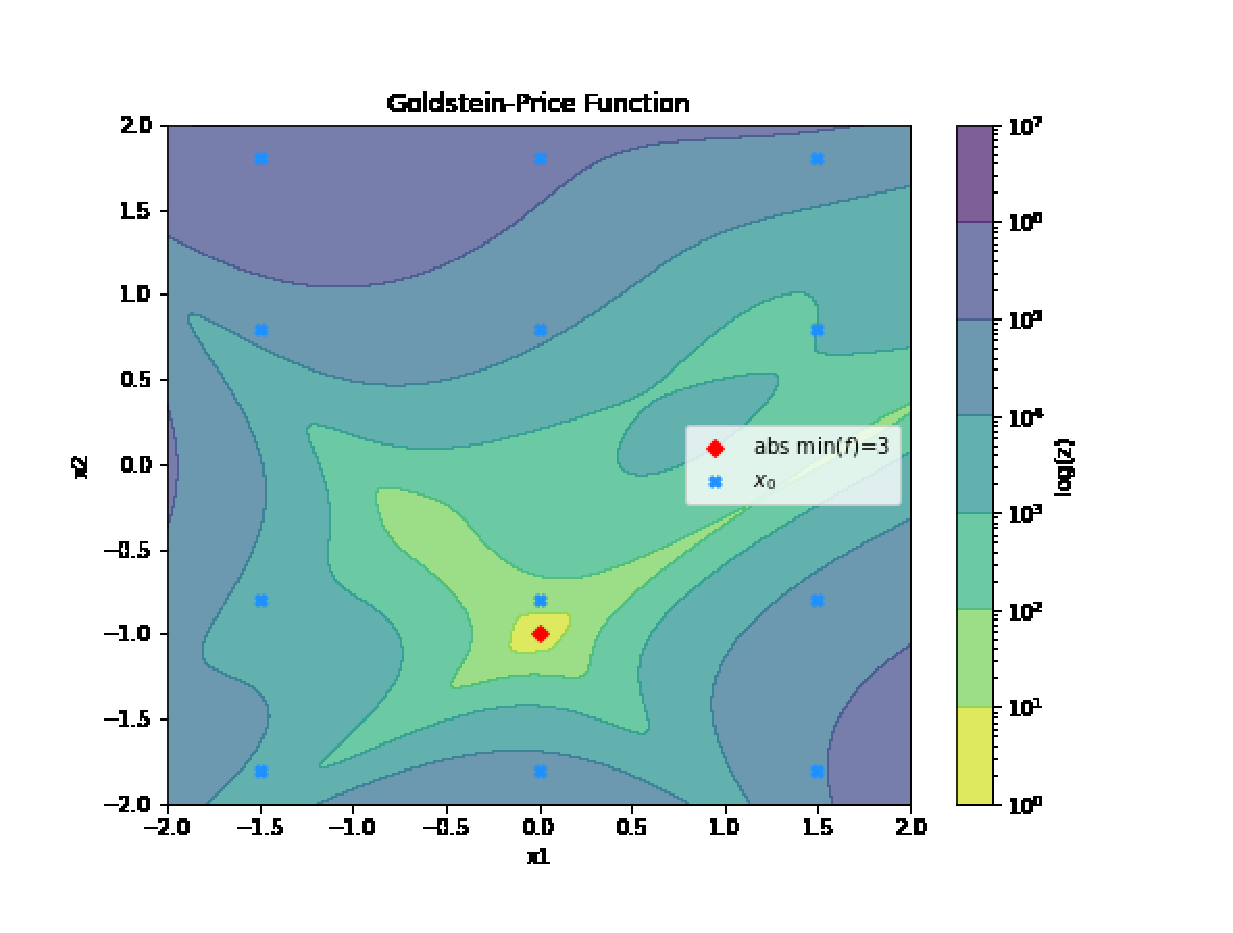
\includegraphics[width=\columnwidth]{figures/pictures/images/goldstein_price-plot2d.eps}
\caption{Goldstein-Price Function}
\label{fig:goldstein_price}
\end{figure}

 The global minimum is located at $x^* = f(0, -1)$ and $f(x^*) = 3$ and labeled with a diamond in \autoref{fig:goldstein_price}.  The domain of the Goldstein-Price function used in this project is restricted to (-2,2) along both $x_1$ and $x_2$ dimensions.  There are 12 regularly sampled points superimposed on \autoref{fig:goldstein_price} and labeled as $x_0$ that are used to initialize separate trials of each optimization algorithm.

\subsection{Bartels-Conn Function}

The Bartels-Conn function \cite{Jamil:2013:CoRR} shown in \autoref{fig:bartels_conn} is characterized by a central elliptical valley with discontinuities appearing at all points along the descent direction.

\begin{equation}
f(x_1, x_2) =  |x_1^2 + x_2^2 + x_1 x_2| + |\sin(x_1)| + |\cos(x_2)|
\end{equation}

\begin{figure}[tb]
\centering
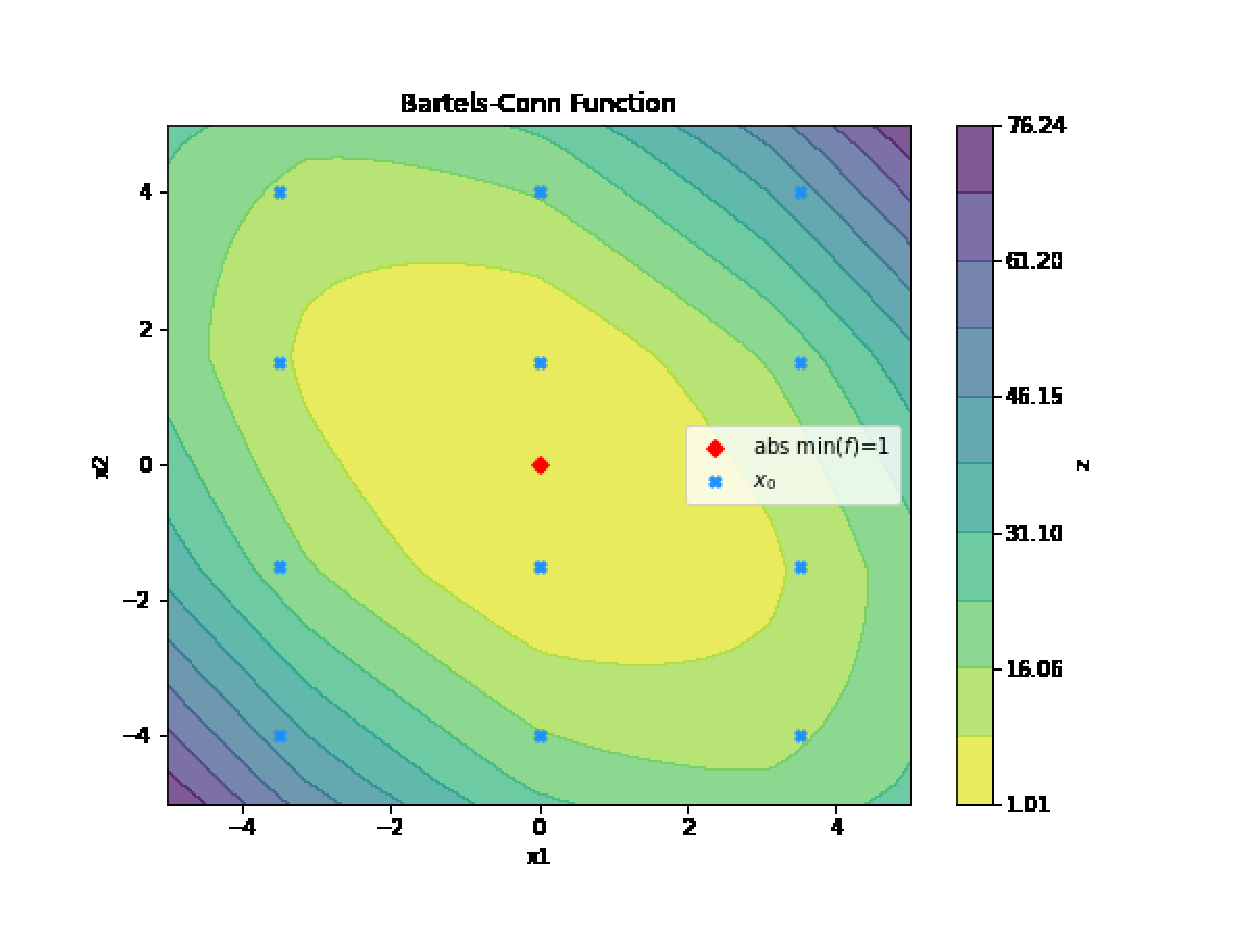
\includegraphics[width=\columnwidth]{figures/pictures/images/bartels_conn-plot2d.eps}
\caption{Bartels-Conn Function}
\label{fig:bartels_conn}
\end{figure}

The global minimum is located at $x^* = f(0, 0)$ and $f(x^*) = 1$ and labeled with a diamond in \autoref{fig:bartels_conn}.  The domain of the Bartels-Conn function used in this project is restricted to (-5,5) along both $x_1$ and $x_2$ dimensions.  There are 12 regularly sampled points superimposed on \autoref{fig:bartels_conn} and labeled as $x_0$ that are used to initialize separate trials of each optimization algorithm.

\subsection{Egg Crate Function}

The Egg Crate function \cite{Jamil:2013:CoRR} show in \autoref{fig:egg_crate} is characterized by many local minima arranged in a two-dimensional grid.  The minimum value of each local minima becomes progressively lower as you move towards the origin.

\begin{equation}
f(x_1, x_2) = x_1^2 + x_2^2 + 25 (\sin^2(x_1) + \sin^2(x_2))
\end{equation}

\begin{figure}[tb]
\centering
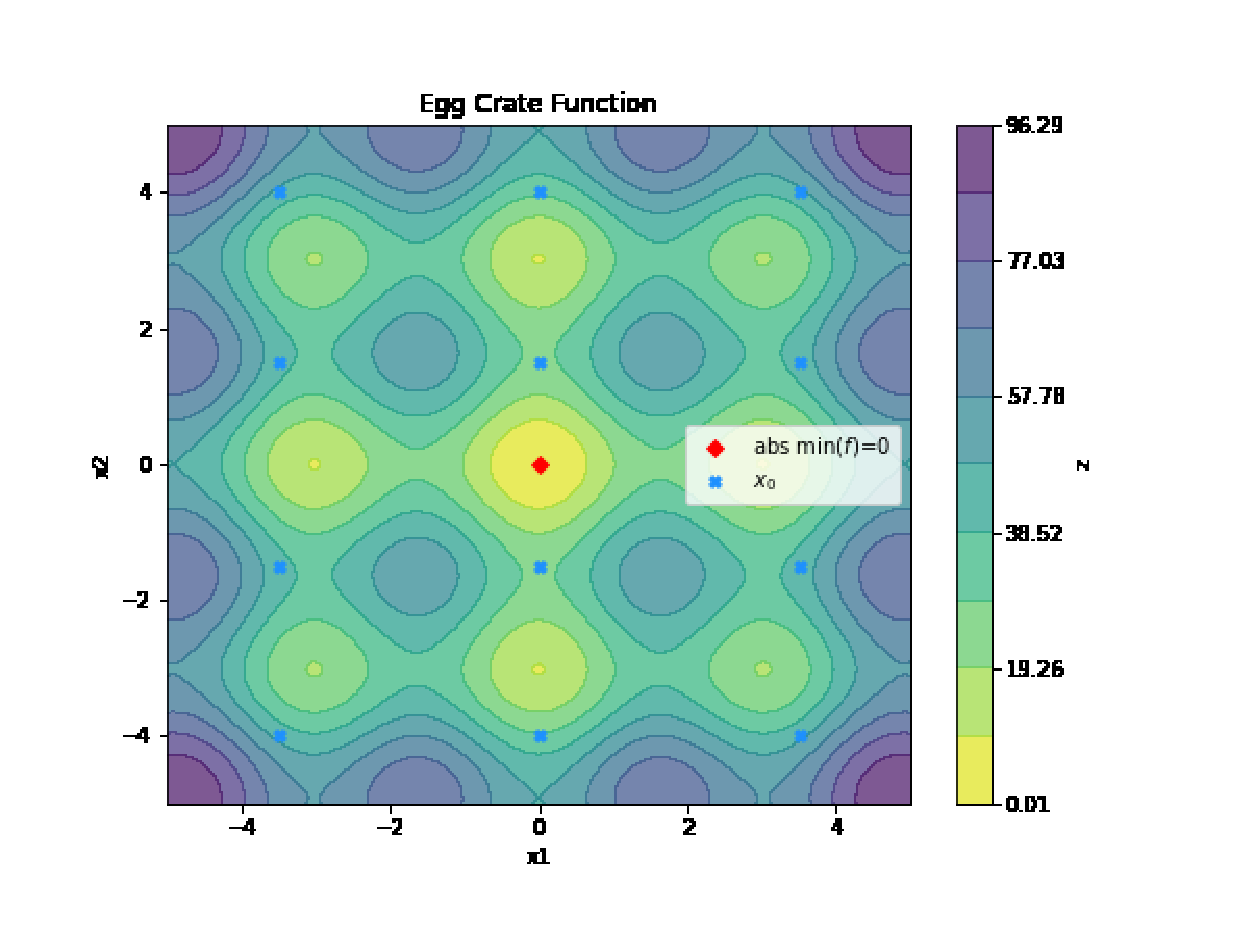
\includegraphics[width=\columnwidth]{figures/pictures/images/egg_crate-plot2d.eps}
\caption{Egg Crate Function}
\label{fig:egg_crate}
\end{figure}

The global minimum is located at $x^* = f(0, 0)$ and $f(x^*) = 0$ and labeled with a diamond in \autoref{fig:egg_crate}.  The domain of the Egg Crate function used in this project is restricted to (-5,5) along both $x_1$ and $x_2$ dimensions.  There are 12 regularly sampled points superimposed on \autoref{fig:egg_crate} and labeled as $x_0$ that are used to initialize separate trials of each optimization algorithm.

\section{Optimization Algorithms}

\autoref{tab:algo_class} summarizes the algorithms used in the project. Each algorithm is classified according to criteria that are based on the description of algorithms for optimzation provided in Kochenderfer and Wheeler (2019) \cite{Kochenderfer:2019}.

\begin{itemize}
\item Gradient-based
	\begin{itemize}
    	\item Gradient-based methods use the derivative of the function to decide on a search direction.  These methods are further subcategorized into whether they use only first-order or second-order information.
    	\item Gradient-based methods are restricted to unimodal or nearly unimodal test functions such as Rosenbrock and Goldstein-Price.
	\end{itemize}
\item Stochastic
	\begin{itemize}
    	\item Stochastic optimization methods incorporate randomness when deciding on a search direction or distance.  Unlike gradient-based methods, these methods are not deterministic and evaluating their behavior is more challenging.
    	\item Although simulated annealing and particle swarm use drastically different search methods (each is described in more detail later), the contrast to make here is between a stochastic method that explores from a single point versus a stochastic method that explores from multiple points in parallel. For these reasons we refer to simulated annealing as a stochastic serial method and particle swarm as a stochastic parallel (or population) method.
    	\item Stochastic methods are not restricted to any test functions.
	\end{itemize}
\end{itemize}

\begin{table}[tb]
	\caption{Algorithm Classification}
    \label{tab:algo_class}
	\scriptsize
	\centering
	\begin{tabu}{
	  r
	  *{7}{c}
	  *{2}{r}
	}
  	\toprule
        Algorithm & Approach \\
	\midrule
        Gradient Descent & Gradient-Based, First-Order \\
        BFGS & Gradient-Based, Second-Order \\
        Simulated Annealing & Stochastic, Serial \\
        Particle Swarm & Stochastic, Parallel/Population \\
	\bottomrule
 	\end{tabu}
\end{table}

\subsection{Gradient Descent}

The Gradient Descent method \cite{Kochenderfer:2019} is a first-order iterative optimization algorithm for finding the local minimum of a differentiable function.

\subsubsection{Gradient Descent Algorithm}

\begin{enumerate}
\item Start with some initial guess $x_0$ and learning rate $\alpha$.
\item Update $x_k$ in the direction of negative gradient $x_k = x_{k-1} - \alpha \nabla f(x_{k-1})$.
\item Evaluate the gradient at the new minimum $\nabla f(x_k)$
\item Repeat from step 2 until $\nabla f(x_k) \approx 0$
\end{enumerate}

\subsubsection{Implementation Details}
Gradient descent is implemented using the \href{https://autograd.readthedocs.io/en/latest/index.html}{autograd} automatic differentiation library to compute the gradient of each test function.  A constant learning rate $\alpha$ is used for all iterations of the algorithm.  The algorithm terminates when the norm of the gradient is less than \emph{tol}.

\subsubsection{Gradient Descent: Rosenbrock}

\autoref{fig:gradient_descent-rosenbrock} shows the result of trial \#10 of gradient descent on the Rosenbrock test function. Observe that search direction is perpendicular to the isovalue given by the contour. Although gradient descent quickly finds the narrow valley containing the global minimum, most of the iterations of the algorithm (nit=8288) are spent slowly traveling along this relatively flat surface.

\begin{figure}[tb]
\centering
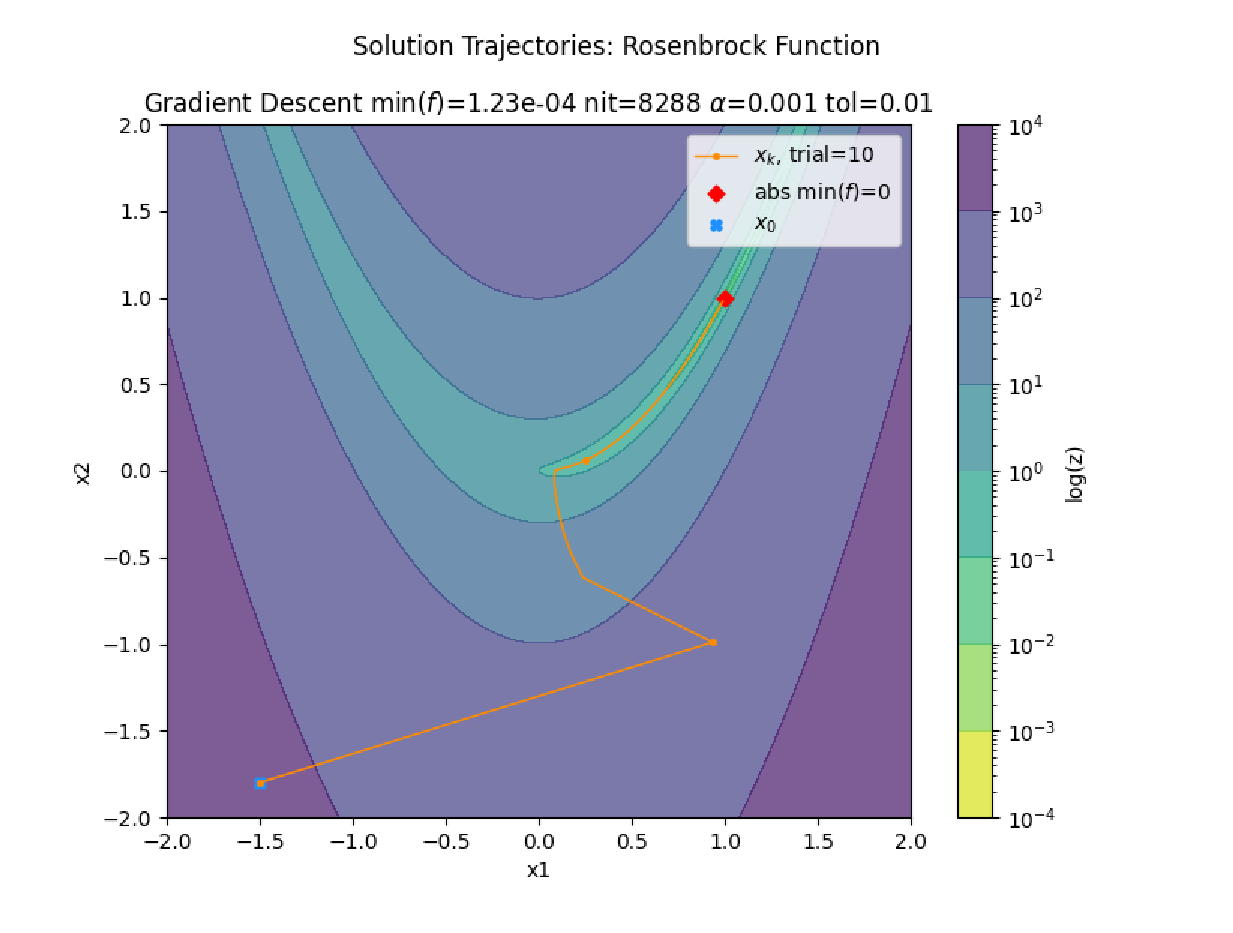
\includegraphics[width=\columnwidth]{figures/pictures/images/gradient_descent-rosenbrock-plot2d-10.eps}
\caption{Gradient Descent on the Rosenbrock Function}
\label{fig:gradient_descent-rosenbrock}
\end{figure}

\subsubsection{Gradient Descent: Goldstein-Price}

\autoref{fig:gradient_descent-goldstein_price} shows the result of trial \#5 of gradient descent on the Goldstein-Price test function. Goldstein-Price is multimodal and as a result, gradient descent is not guaranteed to find the global minimum which is what happens on this trial.  Instead of finding the global minimum, the search ends when finding a flat surface inside of a local minimum ($\min(f)=30$ instead of global $\min(f)=3$).

\begin{figure}[tb]
\centering
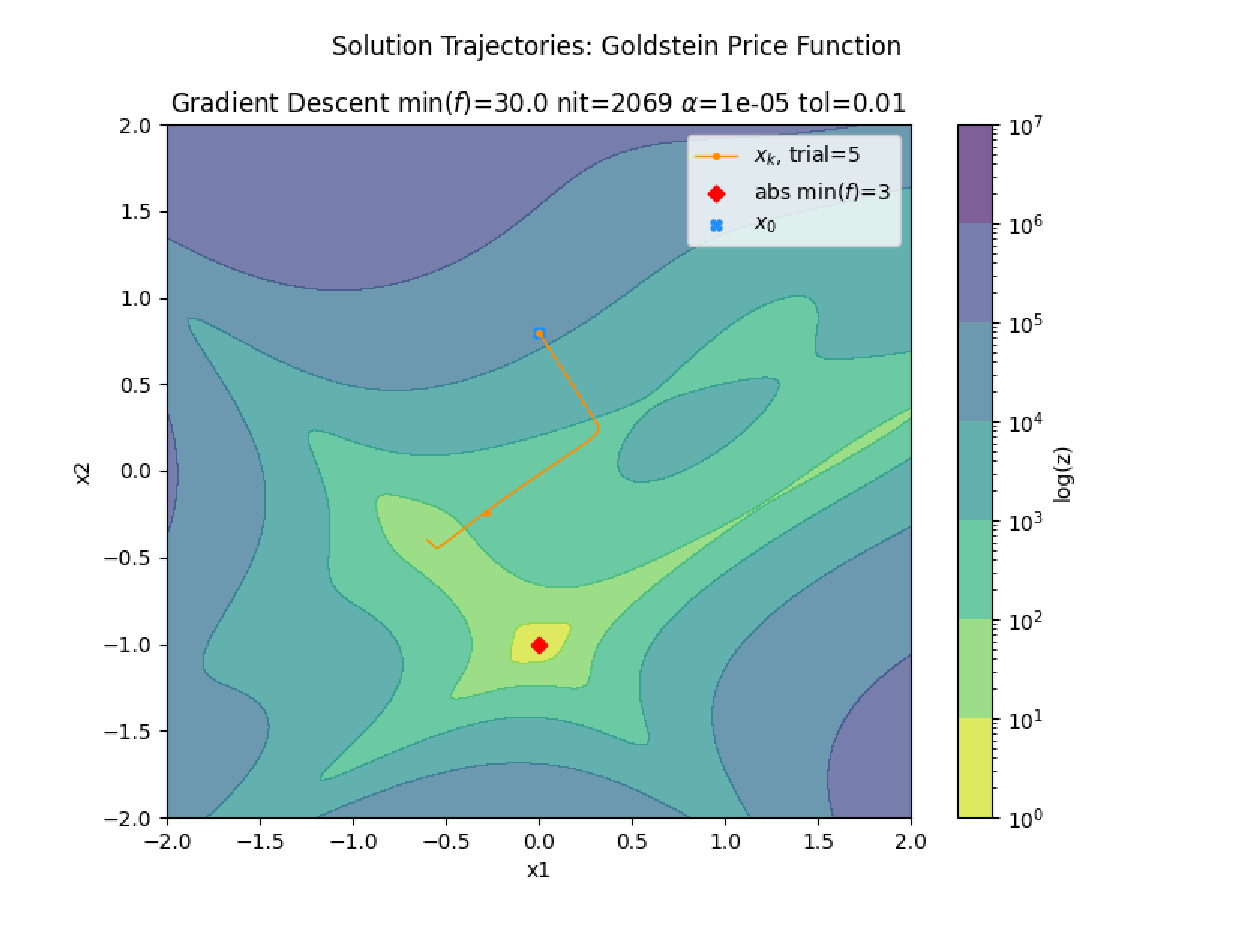
\includegraphics[width=\columnwidth]{figures/pictures/images/gradient_descent-goldstein_price-plot2d-05.eps}
\caption{Gradient Descent on the Goldstein-Price Function}
\label{fig:gradient_descent-goldstein_price}
\end{figure}

\subsection{BFGS}

The Broyden-Fletcher-Goldfarb-Shanno aka BFGS method \cite{Heath:2018} is a second-order iterative optimization method.  The BFGS method is referred to as Quasi-Newton in reference to the fact that unlike Newton's method which uses an explicit Hessian matrix, these methods approximate the Hessian.

$$
x_{k+1} = x_k - \alpha_k B_k^{-1} \nabla f(x_k)
$$

where
\begin{itemize}
\item $B_k$ is approxmation to Hessian
\item $\alpha_k$ is obtained from line search
\end{itemize}

\subsubsection{BFGS Algorithm}

\begin{enumerate}
\item Start with some initial guess $x_0$ and approximate Hessian $B_0 = I$.
\item Solve $B_k s_k = -\nabla f(x_k)$ for $s_k$ or use a line search (described below) to find $s_k$.
\item Compute $x_{k+1} = x_k + s_k$.
\item Compute the difference in gradients $y_k = \nabla f(x_{k+1}) - \nabla f(x_k)$.
\item Update approximate Hessian.
$$
B_{k+1} = B_k + \frac{y_k y_k^T}{y_k^T s_k} - \frac{B_k s_k s_k^T B_k}{s_k^T B_k s_k}
$$
\item Repeat from step 2 until some stopping criteria is reached.
\end{enumerate}

\subsubsection{Implementation Details}

BFGS requires the gradient of the function to minimize and similar to gradient descent the \href{https://autograd.readthedocs.io/en/latest/index.html}{autograd} automatic differentiation library is used to compute the gradient of each test function.  We observed that the performance of the line search has a big impact on the quality of the results obtained and as a result, we replaced a simple version of BFGS written in numpy with a version from scipy having a far more sophisticated line search.  The algorithm terminates when the norm of the gradient is less than \emph{tol}.

\subsubsection{BFGS: Rosenbrock}

\autoref{fig:bfgs-rosenbrock} shows the result of trial \#11 of BFGS on the Rosenbrock test function. Observe that similar to gradient descent the search direction is perpendicular to the isovalue given by the contour. However unlike gradient descent, the line search in the BFGS algorithm is able to exploit second-order information to take larger steps between iterations. As a result, the algorithm converges very quickly (nit=30) in comparison to all the other methods tested.

\begin{figure}[tb]
\centering
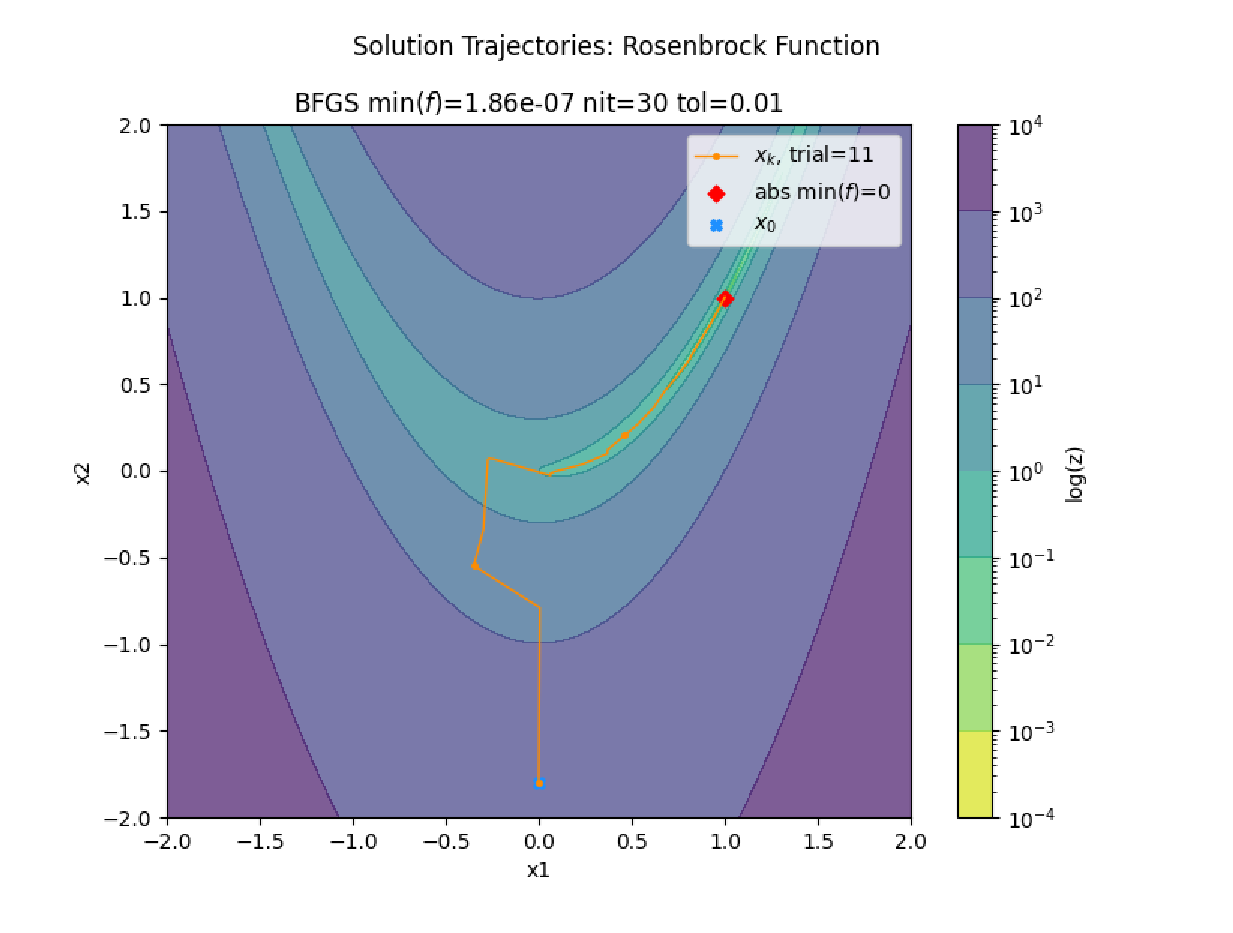
\includegraphics[width=\columnwidth]{figures/pictures/images/bfgs-rosenbrock-plot2d-11.eps}
\caption{BFGS on the Rosenbrock Function}
\label{fig:bfgs-rosenbrock}
\end{figure}

\subsubsection{BFGS: Goldstein-Price}

\autoref{fig:bfgs-goldstein_price} shows the result of trial \#5 of BFGS on the Goldstein-Price test function. Compare this result to the result initialized from gradient descent initialized at the same initial position $x_0$ in \autoref{fig:gradient_descent-goldstein_price}. The solution trajectory used by BFGS avoids passing through the local minimum in which gradient descent was caught. Despite the improvement, BFGS fails to find the global minimum on 6 of the 12 trials of the Goldstein-Price test function.

\begin{figure}[tb]
\centering
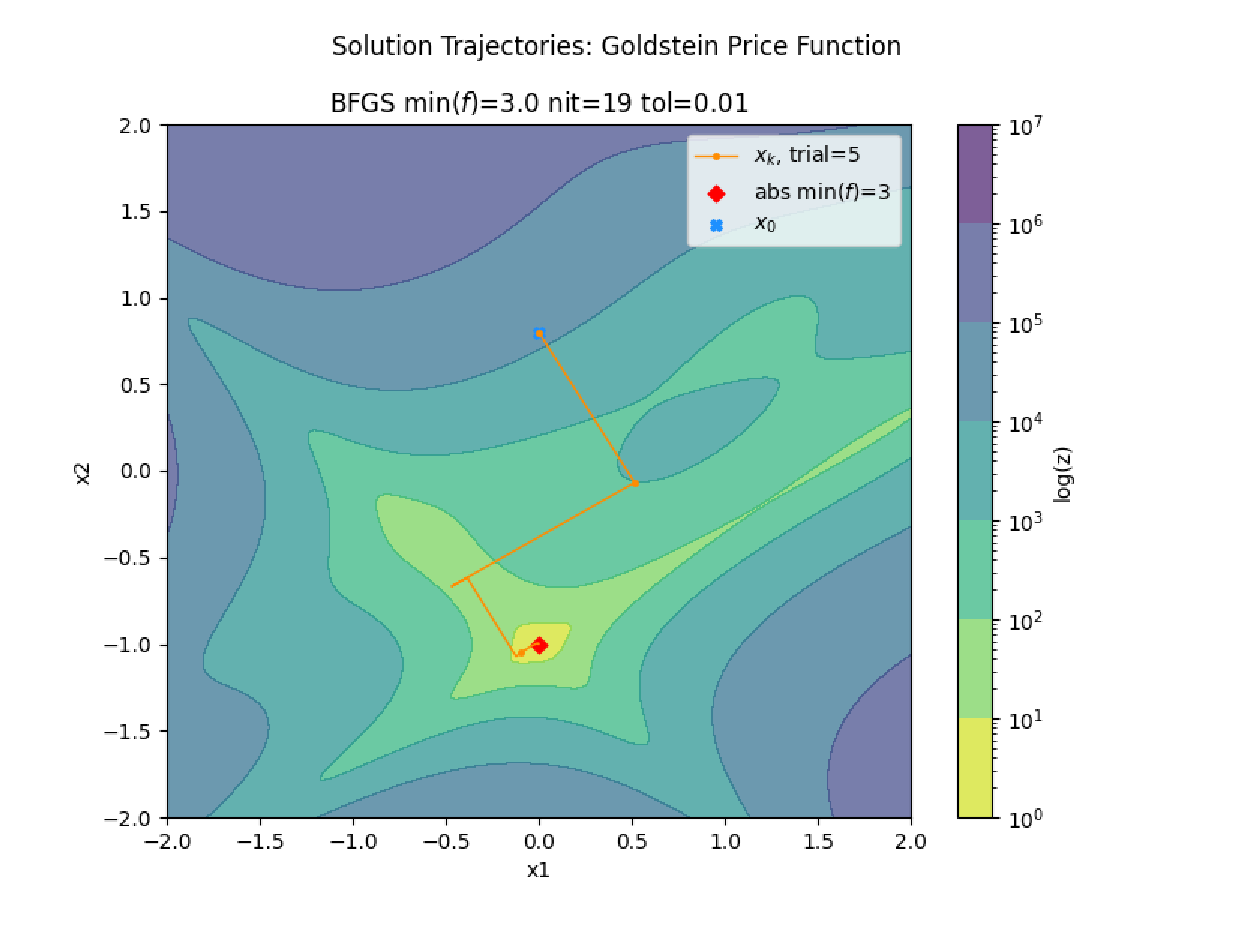
\includegraphics[width=\columnwidth]{figures/pictures/images/bfgs-goldstein_price-plot2d-05.eps}
\caption{BFGS on the Goldstein-Price Function}
\label{fig:bfgs-goldstein_price}
\end{figure}

\subsection{Simulated Annealing}

Simulated annealing \cite{Kochenderfer:2019} is a stochastic optimization method based on the natural physical optimization process that occurs when a material is heated to a relatively high temperature and allowed to cool.  At high temperature the atoms in the material more readily break apart and redistribute allowing the material to become more easily deformed and disordered.  As the material cools, the amount of free energy needed for such motion decreases and the material hardens into an ordered crystal structure.

In the context of optimization, this process suggests two mechanisms:
\begin{itemize}
\item A means by which the search continues in the direction of the local minimum or restarts in a new position that might be initially worse than the current local minimum.
\item A slow decrease in the probability that the algorithm restarts the search in some other position.
\end{itemize}

\subsubsection{Transition Distribution}
The mean and covariance of the transition distribution is used to select a new position.  The new position is described in terms of an offset from the current position according to a multivariate normal distribution.

\subsubsection{Annealing Schedule}
The annealing schedule describes the probability $p(z)$ that the algorithm restarts the search in some other position.  The initial value and rate of decay are parameters of the algorithm.

\subsubsection{Simulated Annealing Algorithm}

\begin{enumerate}
\item Start with some initial guess $x_0$ and set this as the global minimum $f(x_{min}) = f(x_0)$.
\item Generate a new position $x_k$ by adding to $x_{k-1}$ an offset randomly chosen from the transition distribution.
\item Evaluate the function at the new position and compute the change in the objective function $\Delta f(x_k) = f(x_k) - f(x_{k-1})$.
\item If the objective function is improved $\Delta f(x_k) < 0$, then move to the new position, else use the annealing schedule to compute the probability that despite the lack of improvement a change in position is still made.
\item If the function evaluated at this position is less than the global minimum, then update the global minimum $f(x_{min}) = f(x_k)$.
\item Repeat from step 2 until the number of iterations are reached.
\end{enumerate}

\subsubsection{Implementation Details}

Simulated annealing is implemented in numpy with a multivariate normal initialized from a list of means (set to 1. for all trials) and shared covariance matrix (set to the identity matrix for all trials).  Points sampled from this multivariate normal that fall outside of the domain are clipped to the boundary.  More effort could be spent to tune the distribution to each test function, but that wasn't done.  The initial temperature used by the annealing schedule is set to $T_0=1.0$ for all simulations.

\subsubsection{Simulated Annealing: Rosenbrock}

\autoref{fig:simulated_annealing-rosenbrock} shows the result of trial \#10 of simulated annealing on the Rosenbrock test function. The algorithm maintains a history of the absolute minimum that it has found and the location where the algorithm is searching does not necessarily corresond to the algorithm minimum. To help visualize the algorithm progress, the plots and animations of simulated annealing linked from \autoref{tab:anim2d_links} show the evolution of the minimum rather than current location.

\begin{figure}[tb]
\centering
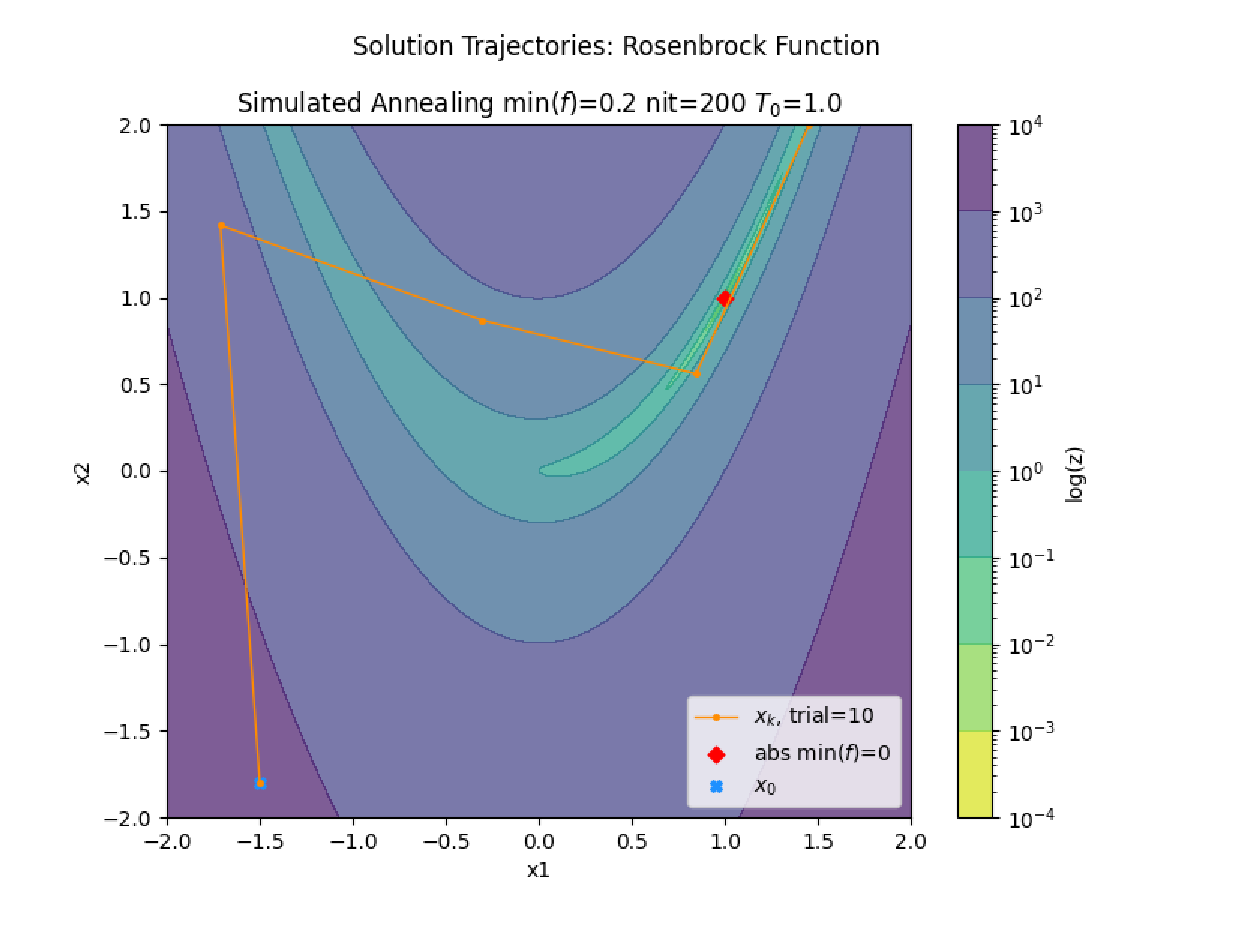
\includegraphics[width=\columnwidth]{figures/pictures/images/simulated_annealing-rosenbrock-plot2d-10.eps}
\caption{Simulated Annealing on the Rosenbrock Function}
\label{fig:simulated_annealing-rosenbrock}
\end{figure}

\subsubsection{Simulated Annealing: Goldstein-Price}

\autoref{fig:simulated_annealing-goldstein_price} shows the result of trial \#6 of simulated annealing on the Goldstein-Price test function. Similar to the previous example, the algorithm does not make rapid progress towards the minimum until about 1000 iterations have passed.

\begin{figure}[tb]
\centering
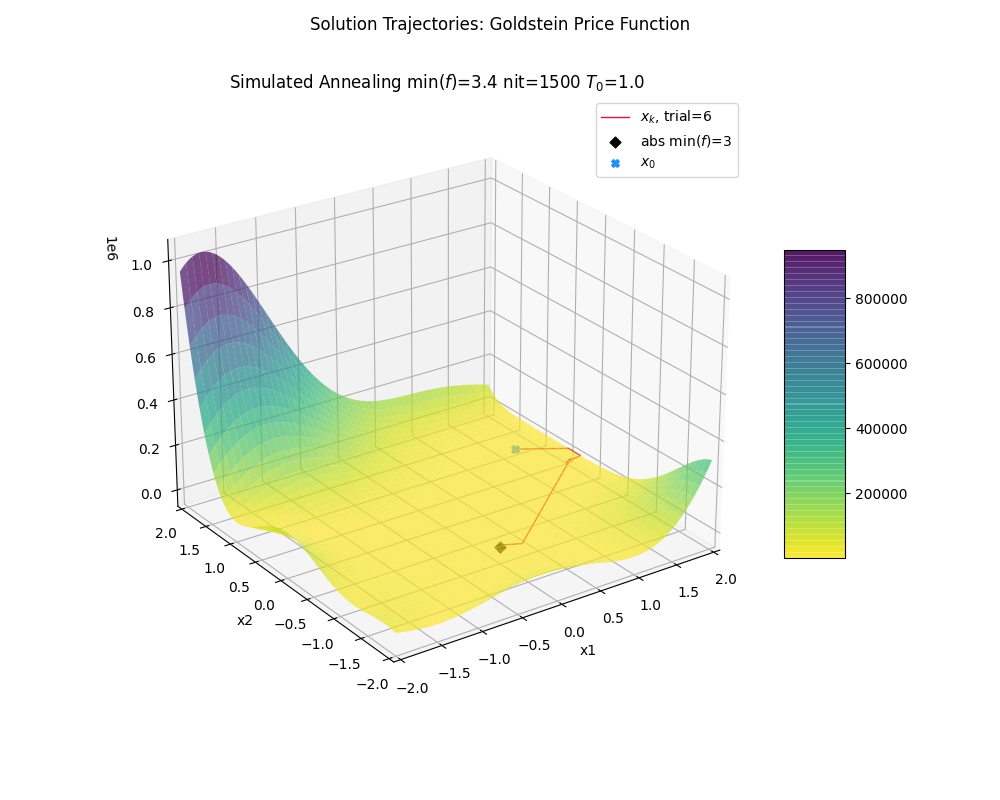
\includegraphics[width=\columnwidth]{figures/pictures/images/simulated_annealing-goldstein_price-plot3d-06.eps}
\caption{Simulated Annealing on the Goldstein-Price Function}
\label{fig:simulated_annealing-goldstein_price}
\end{figure}

\subsubsection{Simulated Annealing: Bartels-Conn}

\autoref{fig:simulated_annealing-bartels_conn} shows the result of trial \#12 of simulated annealing on the Bartels-Conn test function. Since the Bartels-Conn function is not differentiable, we cannot use a gradient-based solver. However, we can compare the progress of the simulated annealing algorithm along the downhill direction of the test surface. In contrast to what we would see from gradient descent or BFGS, the progress downhill zig-zags randomly since there is no gradient information to direct progress. Nevertheless the simulated annealing algorithm finds the global minimum after 200 iterations.

\begin{figure}[tb]
\centering
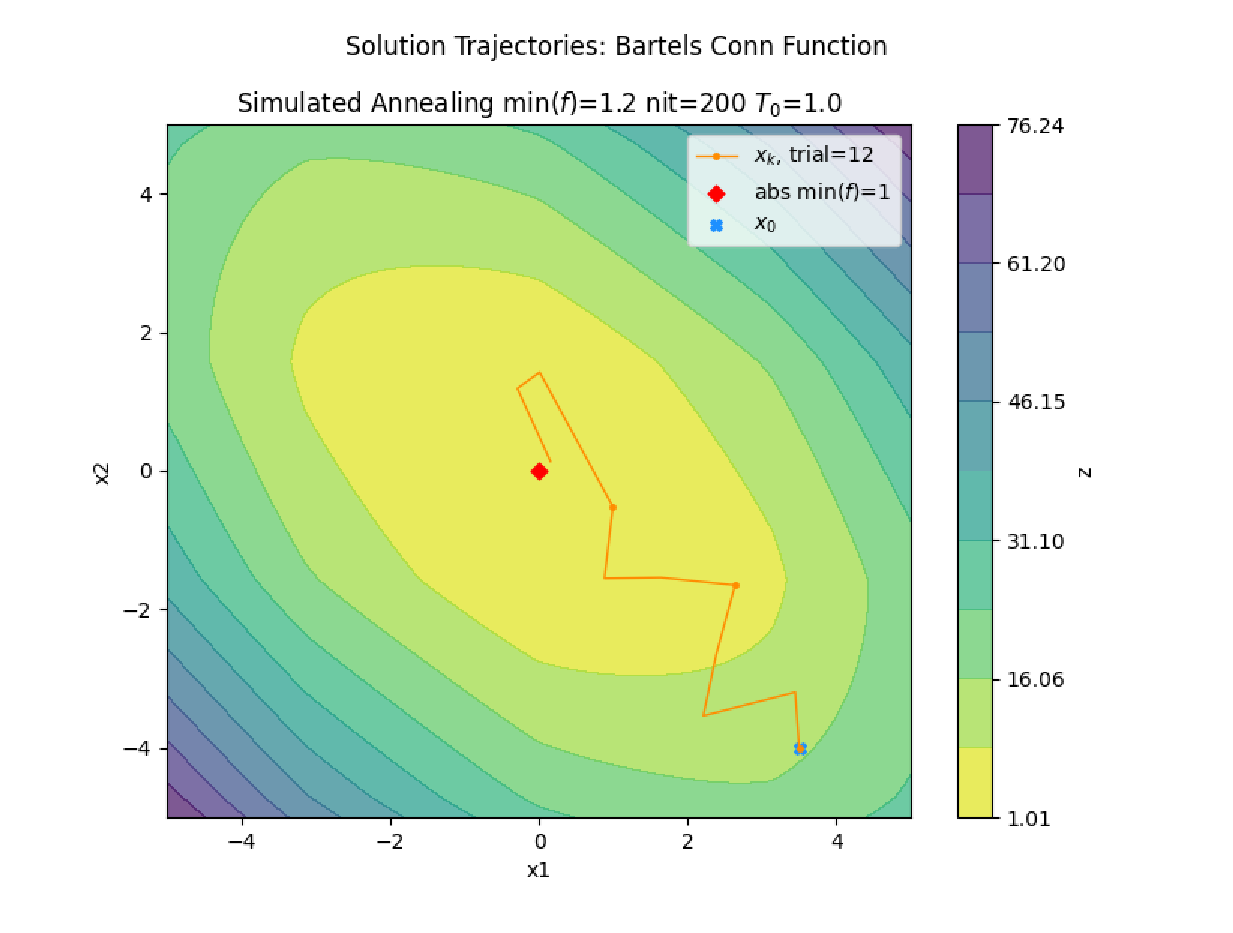
\includegraphics[width=\columnwidth]{figures/pictures/images/simulated_annealing-bartels_conn-plot2d-12.eps}
\caption{Simulated Annealing on the Bartels-Conn Function}
\label{fig:simulated_annealing-bartels_conn}
\end{figure}

\subsubsection{Simulated Annealing: Egg Crate}

\autoref{fig:simulated_annealing-egg_crate} shows the result of trial \#1 of simulated annealing on the Egg Crate test function. This test function has 8 local minima surrounding a global minimum.  The simulated annealing function spends about 1000 iterations exploring 2 of the surrounding local minima before finding the central global minimum.  After so many iterations, the annealing process will discourage restarts and the algorithm spends another 500 iterations to get within 2 decimal places of accuracy ($\min(f)=2.06e-02$) of the global minimum.

\begin{figure}[tb]
\centering
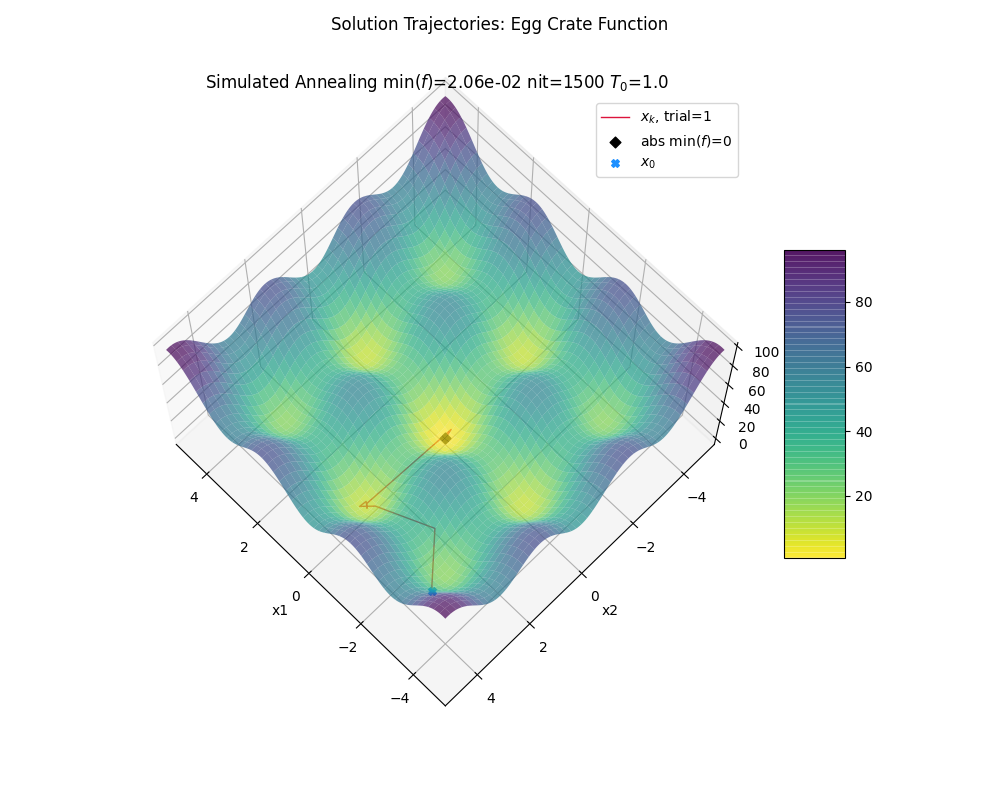
\includegraphics[width=\columnwidth]{figures/pictures/images/simulated_annealing-egg_crate-plot3d-01.eps}
\caption{Simulated Annealing on the Egg Crate Function}
\label{fig:simulated_annealing-egg_crate}
\end{figure}

\subsection{Particle Swarm}

Particle swarm \cite{Kennedy:2001} is a stochastic optimization method based on particles at different positions that simultaneously explore the optimization function and influence each other's search.

Each particle in the swarm is characterized by the following properties:
\begin{itemize}
\item current position
\item current velocity
\item position of the minimum found by this particle
\end{itemize}

The rule that each particle uses to update its' next position is based on the following:
\begin{itemize}
\item current velocity of the particle
\item velocity in the direction of the minimum found by this particle so far
\item velocity in the direction of the global minimum found by all particles so far
\end{itemize}

\subsubsection{Particle Swarm Algorithm}

\begin{enumerate}
\item Initialize a list of $n \times p$-dimensional particles with a random initial position $(x_{1,0}, \cdots, x_{n,0})$ and random velocity $(v_{1,0}, \cdots, v_{n,0})$.
\item For each particle save the position and minimum function value found by that particle $(x_{1,\min}, \cdots, x_{n,\min})$ and $(f(x_{1,\min}), \cdots, f(x_{n,\min}))$.
\item Save the global position and minimum function value $x_{min}$ and $f(x_{min})$.
\item Initialize a counter $k=1$ used to track the iteration number.
\item Update the velocity of each particle for the current iteration $v_{i,k} = \omega v_{i,k-1} + p_1 r_{i,1} (x_{i,\min} - x_{i,k-1}) + p_2 r_{i,2} (x_{min} - x_{i,k-1})$ where $\omega$ is a inertia constant, $p_1, p_2$ are momentum constants, and $r_{i,1}, r_{i,2}$ are per-particle random numbers in the range $[0,1]$.
\item Update the position of each particle for the current iteration $x_{i,k} = x_{i,k-1} + v_{i,k}$.
\item Evaluate the objective function at each new position and update the per-particle and global minimum function values and position.
\item Repeat from step 4 until the number of iterations are reached.
\end{enumerate}

\subsubsection{Implementation Details}

Particle swarm is implemented in numpy. There are a few algorithm hyperparameters which are set to default values for all trials:
\begin{itemize}
\item $\omega$ inertia coefficient (default: 1.0)
\item $p_1$ momentum coefficient towards min position of current particle (default: 1.0)
\item $p_2$ momentum coefficient towards min position among all particles (default: 1.0)
\end{itemize}

An additional hyperparamter controls the number of particles $n$ used in the swarm.  Each particle will participate in the search during an iteration.  As a result, the effective number of iterations of the algorithm is the number of particles multiplied by the number of iterations.  The effective number of iterations (nit) is shown in the plots (the animations of particle swarm linked from \autoref{tab:anim2d_links} have a per-particle iteration counter that ends at nit/n).

Based on experiments adjusting the value of $n$ such that the effective number of iterations is held constant, we observed that the algorithm will always find the global minimum when $n \geq 5$.  A value of $n=3$ was chosen so that the algorithm doesn't always find the global minimum.

\subsubsection{Particle Swarm: Rosenbrock}

\autoref{fig:particle_swarm-rosenbrock} shows the result of trial \#5 of particle swarm on the Rosenbrock test function.  To help visualize the algorithm progress, the plots and animations of particle swarm linked from \autoref{tab:anim2d_links} show the trajectory of each particle rather than the value of the minimum position among all the particles (note the difference in convention compared to simulated annealing).

For this trial $n=3$ particles start from different initial positions that are well dispersed across the test function.  One of the consistent patterns that emerges from the animations of particle swarm linked from \autoref{tab:anim2d_links} is the tendency for particles to converge.  In this trial, all particles converge at the entrance of the narrow valley leading to the global minimum.  Since the particles have only 50 iterations each, there isn't enough time to get closer.

\begin{figure}[tb]
\centering
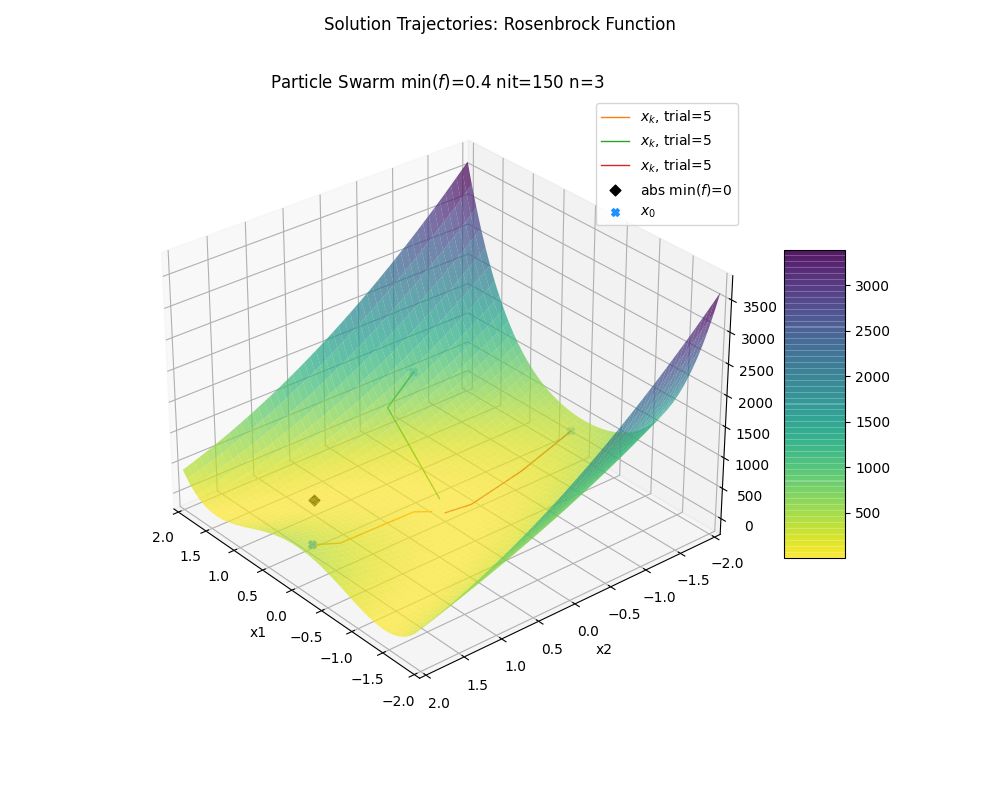
\includegraphics[width=\columnwidth]{figures/pictures/images/particle_swarm-rosenbrock-plot3d-05.eps}
\caption{Particle Swarm on the Rosenbrock Function}
\label{fig:particle_swarm-rosenbrock}
\end{figure}

\subsubsection{Particle Swarm: Goldstein-Price}

\autoref{fig:particle_swarm-goldstein_price} shows the result of trial \#8 of particle swarm on the Goldstein-Price test function. Compare this to the result obtained from BFGS on Goldstein-Price in \autoref{fig:bfgs-goldstein_price}.  Although none of the particles start as close to the global minimum, the collection of particles are able to influence each other such that they all move in the same direction down the slope.

\begin{figure}[tb]
\centering
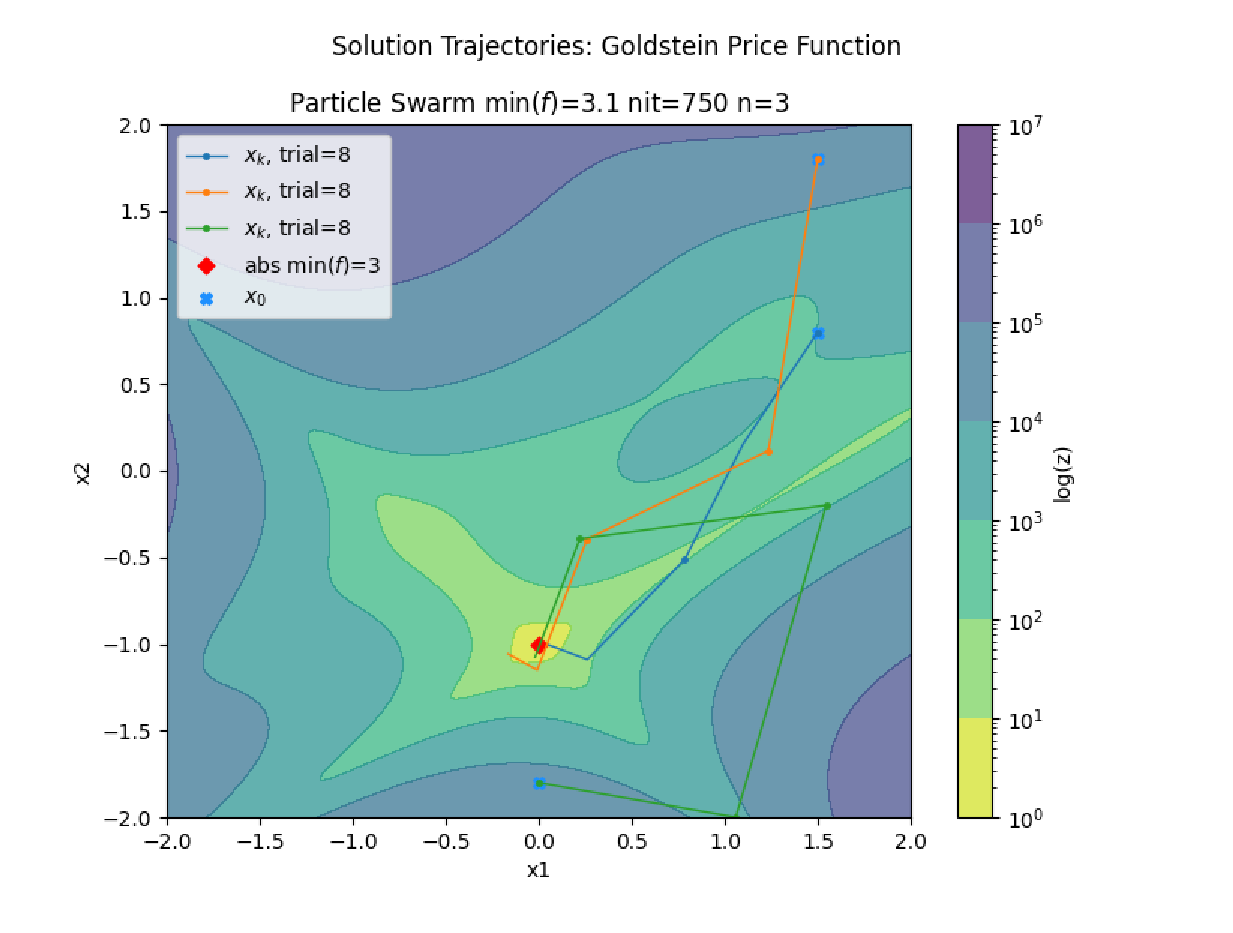
\includegraphics[width=\columnwidth]{figures/pictures/images/particle_swarm-goldstein_price-plot2d-08.eps}
\caption{Particle Swarm on the Goldstein-Price Function}
\label{fig:particle_swarm-goldstein_price}
\end{figure}

\subsubsection{Particle Swarm: Bartels-Conn}

\autoref{fig:particle_swarm-bartels_conn} shows the result of trial \#2 of particle swarm on the Bartels-Conn test function.  In the animation of this trial linked from \autoref{tab:anim2d_links}, two of the particles converge and search together for about 10 iterations (k=36) to find a better minimum at which point they are joined by the third particle at (k=46) until reaching the maximum number of iterations configured for the trial.

\begin{figure}[tb]
\centering
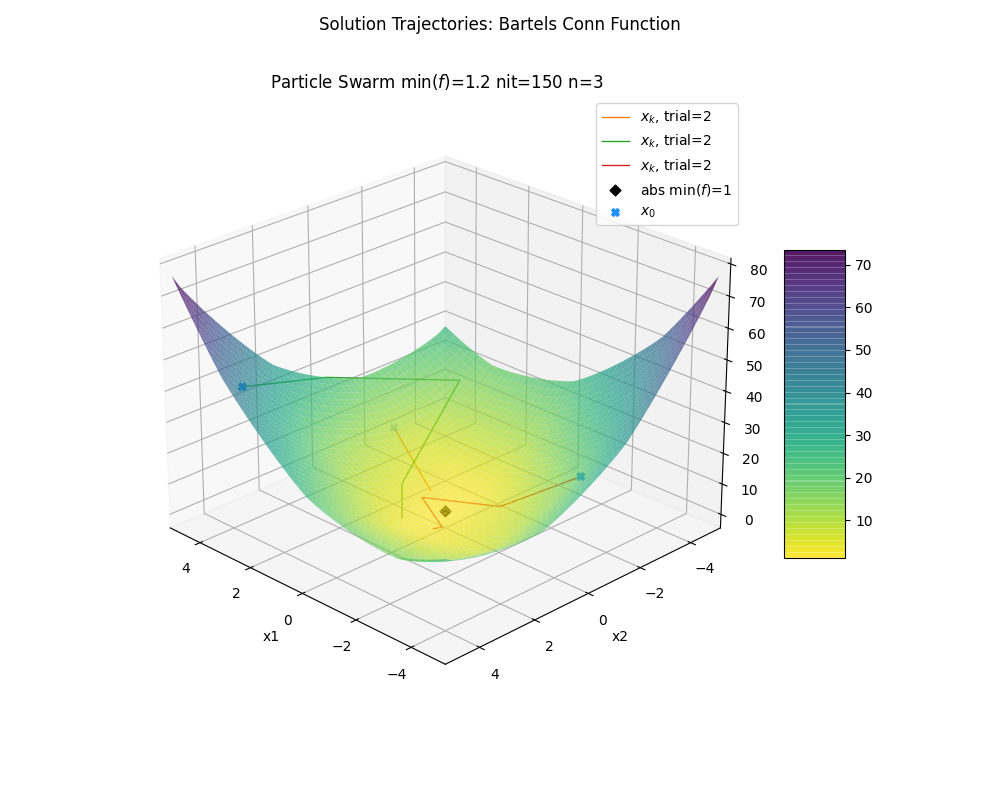
\includegraphics[width=\columnwidth]{figures/pictures/images/particle_swarm-bartels_conn-plot3d-02.eps}
\caption{Particle Swarm on the Bartels-Conn Function}
\label{fig:particle_swarm-bartels_conn}
\end{figure}

\subsubsection{Particle Swarm: Egg Crate}

\autoref{fig:particle_swarm-egg_crate} shows the result of trial \#11 of particle swarm on the Egg Crate test function. The animation of particle swarm for this trial linked from \autoref{tab:anim2d_links} is an excellent demonstration of particles starting from opposite corners of the domain converging and moving together to reach the global minimum.

\begin{figure}[tb]
\centering
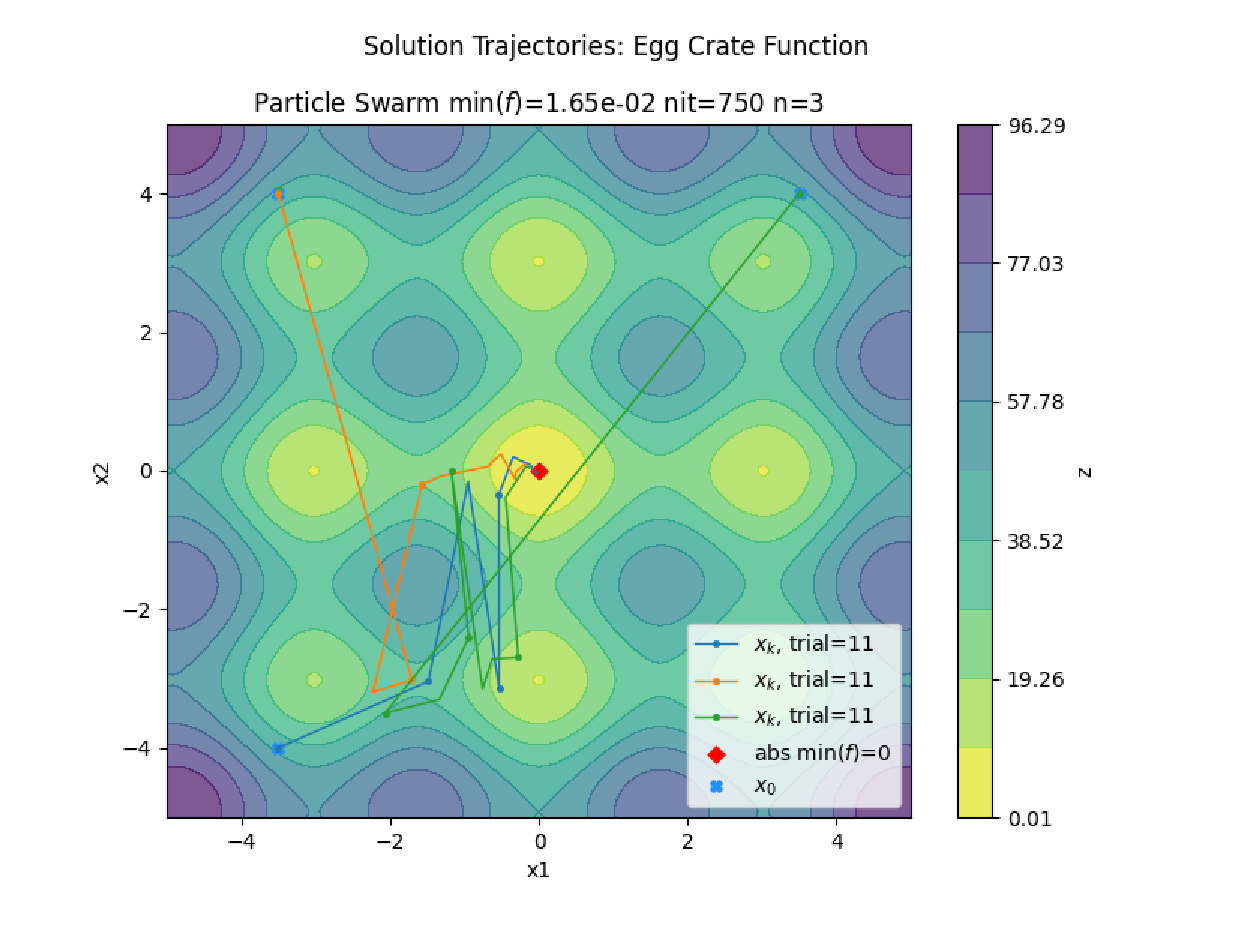
\includegraphics[width=\columnwidth]{figures/pictures/images/particle_swarm-egg_crate-plot2d-11.eps}
\caption{Particle Swarm on the Egg Crate Function}
\label{fig:particle_swarm-egg_crate}
\end{figure}

\section{Results}

\autoref{tab:algo_eval_sum} summarizes the results obtained from running 12 trials of each combination of algorithm and test function. The columns in this table are defined as:

\begin{itemize}
\item alg
\begin{itemize}
	\item Name of algorithm.
\end{itemize}
\item func
\begin{itemize}
	\item Name of test function.
\end{itemize}
\item ntrials
\begin{itemize}
	\item Number of trials.
\end{itemize}
\item nmin
\begin{itemize}
	\item Number of trials reaching minimum (or near-minimum) threshold.
	\item For the Rosenbrock, Bartels-Conn, and Egg Crate functions, any result with an absolute error less than 1.0 from the test surface minimum is considered to have reached the minimum.
	\item For the Goldstein-Price function the same rule applies, but the threshold is 10.0 due to the magnitude of the range across the test function.
\end{itemize}
\item mae
\begin{itemize}
	\item Mean average absolute error of all trials.
	\item The absolute error is computed by taking the magnitude of the difference between the minimum reported by the algorithm and the known global minimum value of the test function.
\end{itemize}
\item mnit
\begin{itemize}
	\item Mean number of iterations to reach a solution.
    \item Gradient-based algorithms will terminate at convergence, but the other algoritms are run for a fixed number of iterations.
	\item Particle swarm uses multiple particles running in parallel. The number of iterations reported for this algorithm in the table reflects the number of iterations of the algorithm multiplied by number of particles.  This makes the number of iterations of this algorithm comparable to a serial algorithm such as simulated annealing.
\end{itemize}
\item msec
\begin{itemize}
	\item Mean elapsed runtime (in seconds) across all trials.
    \item Running time values are reported using a laptop from early 2015 with 2.9 GHz Dual-Core Intel i5 processor and 8GB of memory. The operating system used is ubuntu 18.04.
\end{itemize}
\item algparm
\begin{itemize}
	\item Algorithm hyperparameters and settings used for all trials.
	\begin{itemize}
		\item Gradient Descent: $\alpha$ is learning rate and \emph{tol} is convergence threshold
		\item BFGS: \emph{tol} is convergence threshold
		\item Simulated Annealing: $T_0$ is the initial temperature used in the annealing schedule
		\item Particle Swarm: $n$ is the number of particles
	\end{itemize}
\end{itemize}
\end{itemize}

\begin{table*}[h]
\caption{Algorithm Evaluation Summary}
\label{tab:algo_eval_sum}
\begin{tabular}{llrrrrrl}
\toprule
                 alg &             func &  ntrials &  nmin &      mae &  mnit &  msec &                  algparm \\
\midrule
    Gradient Descent &       Rosenbrock &       12 &    12 & 1.23e-04 &  8281 & 11.58 &  $\alpha$=0.001 tol=0.01 \\
    Gradient Descent &  Goldstein Price &       12 &     3 & 2.04e+02 &  2113 & 25.45 &  $\alpha$=1e-05 tol=0.01 \\
                BFGS &       Rosenbrock &       12 &    12 & 2.51e-06 &    28 &  0.38 &                 tol=0.01 \\
                BFGS &  Goldstein Price &       12 &     6 & 1.49e+02 &    16 &  0.58 &                 tol=0.01 \\
 Simulated Annealing &       Rosenbrock &       12 &    12 & 2.21e-01 &   200 &  0.30 &                $T_0$=1.0 \\
 Simulated Annealing &  Goldstein Price &       12 &     7 & 3.65e+01 &  1500 &  1.23 &                $T_0$=1.0 \\
 Simulated Annealing &     Bartels Conn &       12 &    11 & 1.80e+00 &   200 &  0.19 &                $T_0$=1.0 \\
 Simulated Annealing &        Egg Crate &       12 &     6 & 6.40e+00 &  1500 &  1.43 &                $T_0$=1.0 \\
      Particle Swarm &       Rosenbrock &       12 &    10 & 1.23e+00 &   150 &  0.07 &                      n=3 \\
      Particle Swarm &  Goldstein Price &       12 &     9 & 2.24e+01 &   750 &  0.38 &                      n=3 \\
      Particle Swarm &     Bartels Conn &       12 &    11 & 9.21e-01 &   150 &  0.15 &                      n=3 \\
      Particle Swarm &        Egg Crate &       12 &     6 & 2.71e+00 &   750 &  0.43 &                      n=3 \\
\bottomrule
\end{tabular}
\end{table*}

\begin{table*}[h]
\caption{Selected Animated Solutions}
\label{tab:anim2d_links}
\begin{tabular}{llll}
\toprule
        Algorithm & Surface & Trial & Youtube Link \\
\midrule
        BFGS & Rosenbrock & 1 & \url{https://youtu.be/PDk9d_65sHs} \\
        BFGS & Rosenbrock & 11 & \url{https://youtu.be/_HfCZAnnIgI} \\
        BFGS & Goldstein-Price & 4 & \url{https://youtu.be/Y01H7iUr6js} \\
        BFGS & Goldstein-Price & 5 & \url{https://youtu.be/fIyGMrPIsGk} \\
        Simulated Annealing & Rosenbrock & 10 & \url{https://youtu.be/dcKCRAYu-Oo} \\
        Simulated Annealing & Goldstein-Price & 6 & \url{https://youtu.be/AgMDXNWJH24} \\
        Simulated Annealing & Bartels-Conn & 1 & \url{https://youtu.be/wp2_u-zHY7c} \\
        Simulated Annealing & Bartels-Conn & 12 & \url{https://youtu.be/KKK3SiV80Ls} \\
        Simulated Annealing & Egg Crate & 1 & \url{https://youtu.be/bfBrm2unoOg} \\
        Particle Swarm & Rosenbrock & 5 & \url{https://youtu.be/SzwsbCBg-tk} \\
        Particle Swarm & Goldstein-Price & 4 & \url{https://youtu.be/cyyI9hAzjqg} \\
        Particle Swarm & Goldstein-Price & 7 & \url{https://youtu.be/sQjNwbgXpvc} \\
        Particle Swarm & Goldstein-Price & 8 & \url{https://youtu.be/FIHklbjZrQ0} \\
        Particle Swarm & Bartels-Conn & 2 & \url{https://youtu.be/crtcMyoKOzQ} \\
        Particle Swarm & Egg Crate & 10 & \url{https://youtu.be/s9MEM_ML3kg} \\
        Particle Swarm & Egg Crate & 11 & \url{https://youtu.be/Z0m8CiTAb3M} \\
\bottomrule
\end{tabular}
\end{table*}

\section{Conclusion}

The following conclusions can be drawn from the comparative results presented.

When using gradient-based solvers, first-order methods such as gradient descent require more iterations to find the global minimum than second-order methods such as BFGS. Use of a dyanamic learning rate with gradient descent would reduce the number of iterations required, but would not change the fundamental conclusion.

Gradient-based solvers achieve higher levels of accuracy than stochastic solvers. In our tests gradient based solvers achieve about 6 decimal digits of precision on the Rosenbrock function, whereas stochastic solvers achieve at most 1 decimal digit of precision on the same test function despite using more iterations.

Stochastic solvers can sometimes find the global minimum despite getting caught in a local minimum. In contrast, a gradient-based solver cannot escape a local minimum.  In our tests simulated annealing and particle swarm are able to find the global minimum of the Goldstein-Price function more frequently than BFGS and gradient descent. Increasing the number of iterations given to BFGS and gradient descent would not change this outcome.

Stochastic solvers require more iterations than gradient-based solvers, but less computational effort per iteration. The mean runtime per iteration (msec/mnit) of simulated annealing and particle swarm on the Rosenbrock and Goldstein-Price function is less than BFGS and gradient descent.

Particle swarm is more computationally efficient than simulated annealing. Both particle swarm and simulated annealing reached the benchmark on 36 of 48 trials, but particle swarm required 1800 mean number of iterations (mnit) whereas simulated annealing required 3400 mnit.

\section{Future Work}

The following should be considered for future work.

All of the test functions are from $f: \mathbb{R}^2$. Repeating these experiments on higher dimensional test functions could produce different results. Interesting properties to study would be the growth in number of iterations required by the stochastic solvers versus the growth in computational cost of the gradient-based methods on higher dimensional surfaces.

One alternative that wasn't explored by this study is to use repeated trials of stochastic solvers initialized at different initial points rather than increasing the number of iterations from the same initial point.

\bibliographystyle{abbrv-doi}

\bibliography{Optimization-Visualization-mmorais2}

\end{document}

